%\lhead{\sffamily  {\small Dark Energy}}
\lhead{{\small LSST undergraduate internships at Fermilab}}

\section{LSST Data Science Internships at Fermilab}

% For student internship proposals, 
% describe the student or selection process, mentoring strategies, and a summary of the 
% existing internship program if the proposal is to augment that. 

 
We propose to build on last year's successful research mentorship program for undergraduates at the Center for Particle Astrophysics at Fermilab.
Interns will participate in data-driven LSST science projects, implementing data science tools (e.g, statistics, machine learning, data visualization, and high-performance computing) and engaging in training and tutorials on these tools.
Our capabilities in image processing, cosmological modeling, and machine learning combine for a uniquely powerful
data science experience for interns and a research advancement for mentors.
We will also implement regular training for science communication and inculcate best practices in software development.


The 7$^{th}$ floor of Wilson Hall at Fermilab is home to roughly a dozen
experimental astrophysicists that helped build and operate
the revolutionary Sloan Digital Sky Survey, helped build and operate
the evolutionary Dark Energy Survey, and will soon help to operate 
the revolutionary Large Synoptic Survey Telescope. Cosmic surveys are
what the group was founded to do in 1992 and what we've been doing for 25 years.

% The culture here is interesting: for example, the postdocs do not work for
% a supervisor, they are their own independent scientists. Often our job as 
% staffers here at the Lab is to support the postdocs in their 
% ambitious scientific pursuits. The postdocs 
% often produce astounding results- such as Alex Drilca-Wagner's dwarf galaxy searches,
% which  enabled new limits on dark matter. Our current set of postdocs 
% came to the 7th floor to help us extract science from the DES data stream,
% but each are trying to create something new, something of their own or 
% something jointly with a colleague. Now they are looking to the future,
% looking to perform exciting science  inside the DESC science collaboration.
% These postdocs set our science goals: cluster cosmology, dark matter via
% dwarf galaxy studies, strong lensing, machine learning.

The scientific culture here is driven by our outstanding postdocs and mission to support
world-class cosmology experiments. A strong strand in this culture is mentoring
junior scientists, both  as visitors from collaborating institutions and as participants
in various summer programs.
During the summer the population on the 7th floor more than doubles.
Fermilab's Summer Interns in Science and Technology program (SIST),
DOE's Science Undergraduate Laboratory Internship program (SULI), and the University of
Chicago's Metcalf Intern program provide undergraduate students. 
Fermilab's TARGET program brings in the best high school 
students from the Chicagoland area for a summer, 
and our relationship with Illinois Math and Science Academy provides
high school students with a longer term summer program here.
This coming year two graduate students, one from University of Chicago and the
other from the Ohio University, will study here on the DOE Office of Science
Graduate Student Research Program.

Last year the LSSTC Enabling Science grant allowed us to bring in
4 undergraduate interns and 1 lab manager/intern to pursue LSST
cosmology and gravitational wave science. 
Interns worked in teams and alongside those from other internship programs on LSST science projects. 
They used Git to share code, sat in each other's offices to work on problems, and exchanged plots to prepare posters, talks, and reports. 
Peer groups learn from each other,
and differences in experience represent chances to teach: high school
students learn readily from undergraduates, and undergraduates learn
by leading high school students. 
In addition, we piloted a science communication training event with the Fermilab Communications Staff. %: Public Information Office Andre Salles led a 1.5-hour training session.
The interns uniformly self-reported a fantastic experience: each with their strengths,
they felt part of something greater, part of a team building something 
for science. That is, they felt part of the large-collaboration experience.
We believe we should build on this extremely successful experience.

Our candidates were pulled from a wide geographic base and from pools that are diverse in background and identity:
two University of Chicago students, one Grinnell College students, 
one (for the second summer) from Macalester College, and
one from the University of West Virgina. They joined with 7th floor SIST, SULI,
and Metcalf interns and a team visiting from Brandeis University to form
a mentoring laboratory of 3 postdocs, 2 graduate students, 11 undergraduates, and 4
high school students,
supported by 3 senior scientists. The lab manager model worked well for us:
a more experienced student is brought on to help the summer interns
learn how to do relatively introductory activities (and some research mentorship), while post-docs and senior scientists spend
their time mentoring the interns on science and software.
This also helps the lab manager learn skills in group organization and team-building.
%(at Fermilab the exemplar is learning to print)

%For the second summer in a row,
%the experiment of aiming to have the students learn as much from each other as from
%the more senior scientists was encouraging.
In the summer of 2019, we will continue to build the healthy culture of co-work and multiple mentors. 
We will add new elements and structure in training for data science, software development, and science communication.
This summer we will bring a machine learning perspective to last summer's
data science endeavors. 

\newpage

Fermilab is active in the LSST Dark Energy Science Collaboration (DESC) and LSST studies of dark matter.
We will aim the students at studying the DESC DC2 catalogs --- engaging science questions related to strong gravitational lensing, supernova light curve analysis, artifact analysis, all of which are data-science oriented problems. 
The students will take on leadership roles where possible, and will be provided opportunities to contribute to publishable work.
The students will ramp up their activity and obtain experience by re-creating a corpus of plots that are related to their project.
Each step of their research will be scaffolded by effective practices in software development, including the usage of versioning repositories, like Git (and using GitHub's full feature set for software development), as well as unit testing and thorough documentation.
While the students are using data science tools in their research, we will also provide a weekly tutorial session for using machine learning tools.

%the DC2 catalogs, the CosmoSIS cosmological modeling program,
%DESC Jupyter notebooks, Github, and teamwork. Once they have done so,
%we ask them to make an improvement. That simple, and that hard.

%The actual science we have them do is secondary: perhaps it is the
%halo mass function, perhaps it is the galaxy-galaxy correlation function.
%All of these are new to undergraduates, and by doing the classics they
%become ready to do things new.

%We will ask them to ramp up on a machine learning algorithm and
%to learn how to apply it in the context of their problem.

This approach to science reflects our intent to prepare the students to become active scientists
with LSST/DESC science products. 
Large scientific collaborations can have steep learning curves, and laying this groundwork during a summer internship can make students attractive candidates for graduate programs.
Of last year's LSSTC interns, two are applying for graduate school,
one is taking a gap year before applying to graduate school, and one
will be a senior in the fall.
Our aim is to evolve this summer program to meet the needs of junior scientists and help them prepare to thrive in the LSST era. 
There are several components to do this: research, software, and communication. We aim to help interns and scientists develop skills in these critical areas for collaborative science.

To summarize, we  propose to leverage the tradition 
of mentoring at Fermilab by
bringing on four undergraduate interns supported by LSSTC
and several more from existing Fermilab intern programs.
The interns will form a group around a more experience
group manager, and will explore the science
of combining LSST DESC DC2 science analyses with cosmological modeling
under the supervision of experienced cosmic
survey scientists. This  model was shown to be extremely successful last year. 
Many of these undergraduates will
form the candidate graduate student classes in years to come.

\begin{figure}
  \centering
    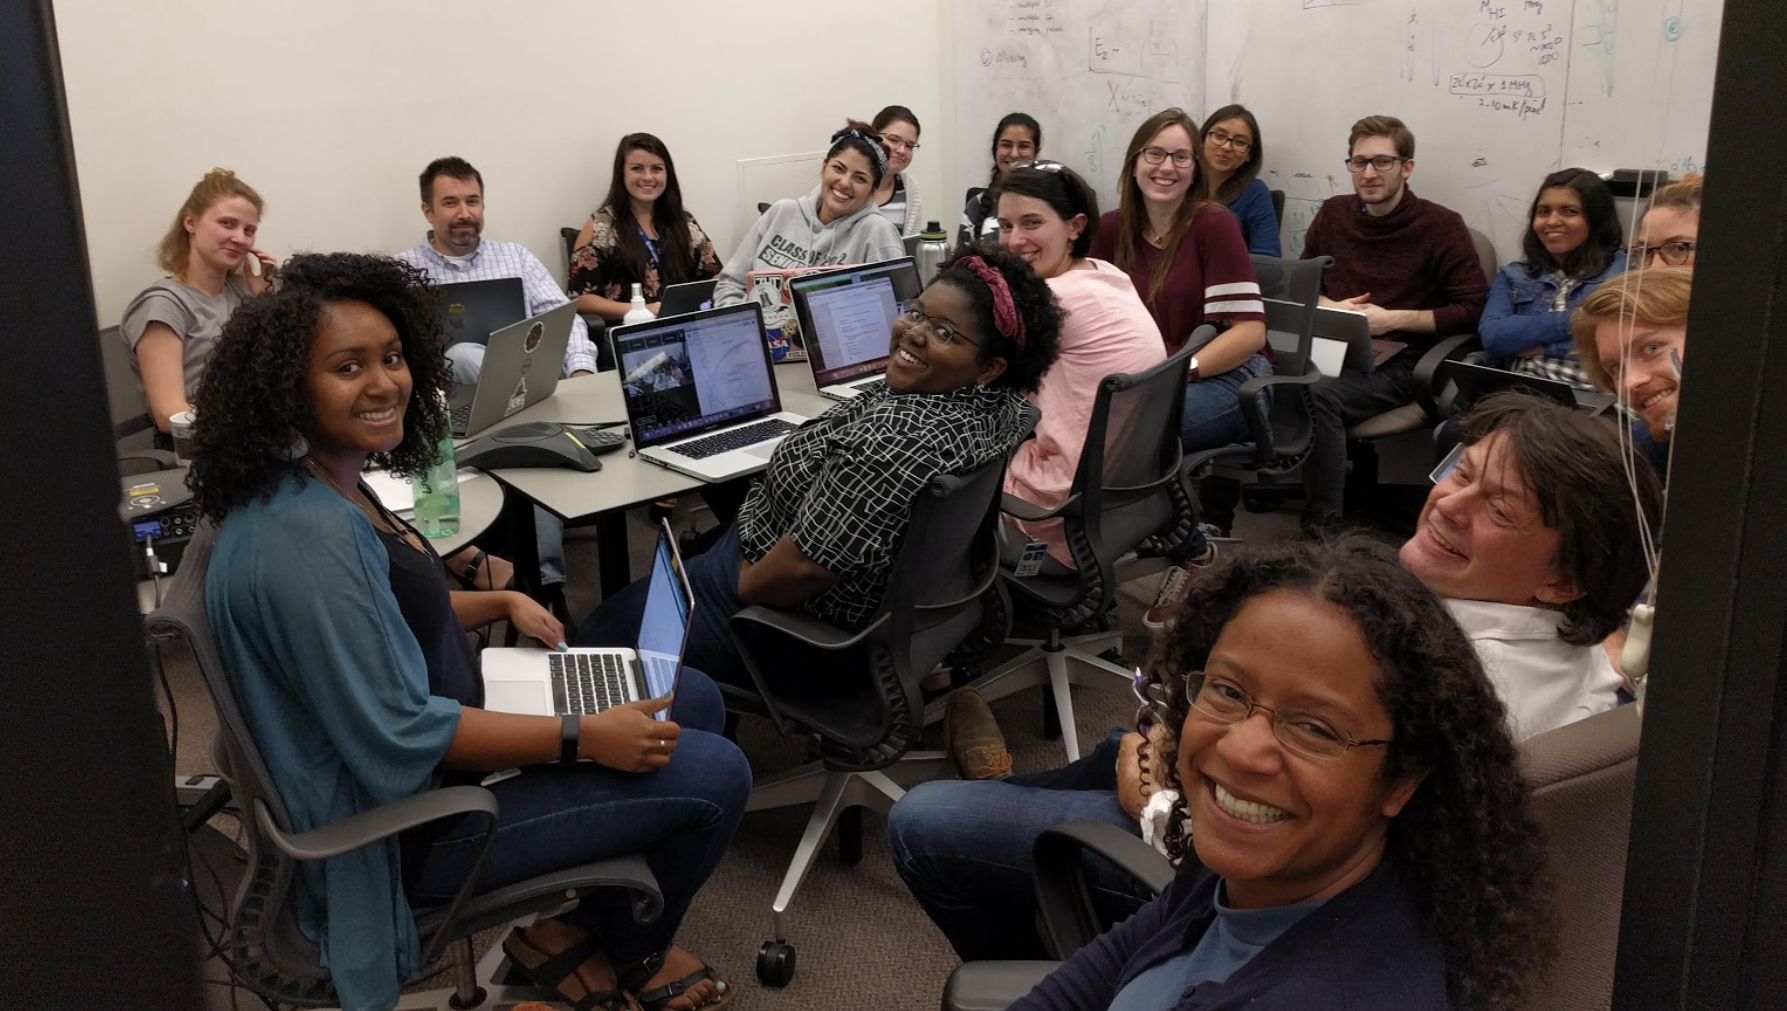
\includegraphics[width=0.66\textwidth]{interns.png}
  \caption*{The summer 2018 intern group at Fermilab's 7th floor, with the 
three senior scientist mentors, one postdoc, and one high school student. 
Three of five of the 2018 LSSTC funded interns are present.}
\end{figure}

\newpage
\section{Intern support and recruitment}

Fermilab has an active internship program. Two internship programs
have been mentioned, and there are four others. The internship
programs here share a Summer Undergraduate Lecture Series run by
Fermilab and visiting scientists, as well as a number of other activities to explore science and careers in cosmology and physics. There is an end-of-summer poster
session given by the summer interns. All of these interns
are housed on or near the lab; we have institutional
experience in handling housing. Lastly, as the US center for
experimental high energy physics, Fermilab itself inspires
the imagination of its interns: they are working at the frontier
of knowledge.

We will continue to recruit interns from diverse and underrepresented groups, 
advertising and engaging through our community connections and national societies (e.g., NSBP, NSHP, oSTEM). 
We will also welcome applications from University of Chicago undergraduates. 
Fermilab has many scientists on joint appointments with
the University of Chicago. There are many more students
requesting research projects then can be supported by 
the University - an opportunity that Fermilab capitalizes on.
Other avenues exist: the Fermilab User community has many undergraduates
from which we could make invitations, 
and Fermilab performs national student selection for many of its summer
intern programs.

For each of our interns, there will be a primary science mentor (not the lab manager). 
We have identified the post-baccalaureate candidate (Andres Felipe Hernandez) who will fulfill the role of lab manager.



